\textbf{Considera el mundo de la aspiradora constituido por dos celdas. Si el agente utiliza el siguiente algoritmo para desempeñar sus funciones:}

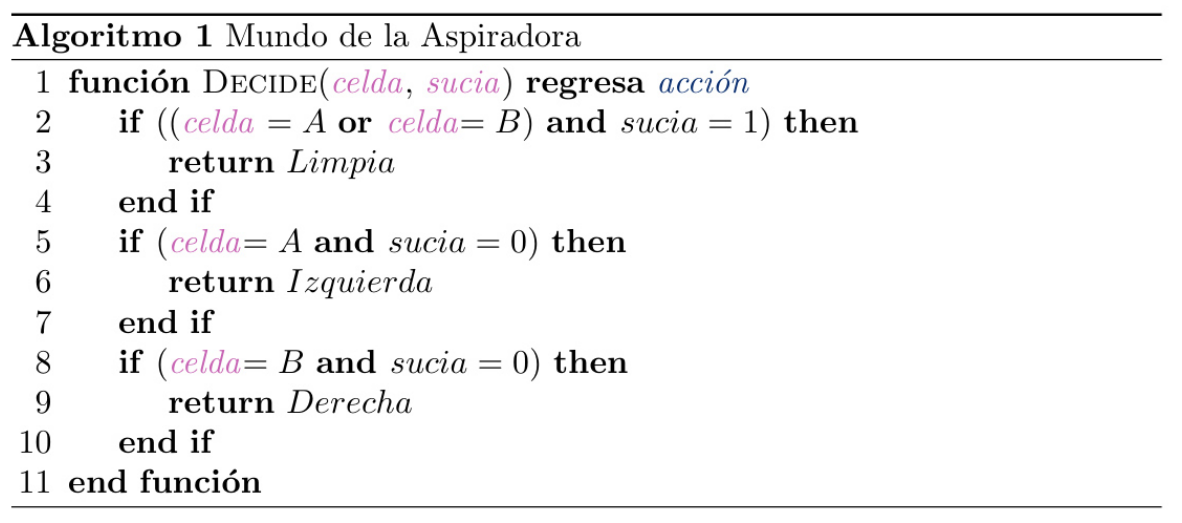
\includegraphics[width=16cm]{src/Img/Screenshot_20250224_024900.png}

indica el tipo de agente en el que podría clasificarse (1 pt.). \vspace{.3cm}

Me parece que la aspiradora es un \textbf{agente reactivo simple}, ya que se basa únicamente en su percepción actual, ignorando lo que haya ocurrido antes o lo que pueda suceder después. Se observa que utiliza condiciones muy simples diseñadas únicamente para evaluar la celda en la que se encuentra. \vspace{.2cm}

Además, considerando que este ambiente solo tiene dos posibles estados de suciedad y que las únicas acciones disponibles son moverse de casilla o limpiar, este modelo es bastante adecuado y debería cumplir su función de manera más o menos efectiva (nótese que si no hay suciedad, la aspiradora estará en un ciclo constante de movimiento de un lado a otro).  
